
\chapter{Format danych wejściowych}

Problem rozwiązywania planu zajęć jest zagadnieniem popularnym w świecie naukowym. Dostępnych jest wiele rozwiązań i ciągle powstają nowe. Jednak, by móc porównać ze sobą dwa różne algorytmy, konieczne jest operowanie na tych samych danych testowych. Z tego powodu naukowcy uzgodnili wspólny format danych wejściowych o nazwie XHSTT i stworzyli bazę danych wraz z przykładowymi rozwiązaniami \cite{Database}. Dane te zapisane są z wykorzystaniem języka XML. Format XHSTT ma duży stopień skomplikowania, dlatego postanowiono poświęcić cały rozdział na jego opisanie \cite{XHSTT}. 

\section{Budowa archiwum}

Archiwum jest kolekcją instancji zawierających dane dla problemu układania planu zajęć, razem z potencjalnymi grupami rozwiązaniami. Każda grupa rozwiązań zawiera rozwiązania dla jednej instancji z archiwum. Ogólny szablon dokumentu przedstawiono na rysunku 4.1. 

\begin{figure}
	\centering
	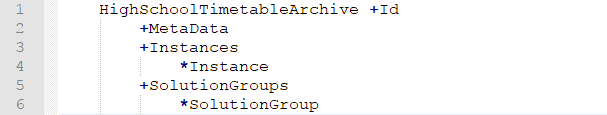
\includegraphics {szablonXHSTT}
	\caption{Szablon archiwum XHSTT.}
	\label{fig: szablonXhstt}
\end{figure}

W tej notacji, słowa znajdujące się w tej samej linii oznaczają, że pierwsze  słowo jest nazwą kategorii, a kolejne słowa to jej atrybuty. Słowa umieszczone poniżej w zagłębieniach to nazwy podkategorii. Znak + przed nazwą oznacza, że kategoria lub atrybut jest czymś opcjonalnym. Znak * oznacza, że dana kategoria może wystąpić zero lub więcej razy. Przykład w formacie XML zaprezentowano na rysunku 4.2.

\begin{figure}
	\centering
	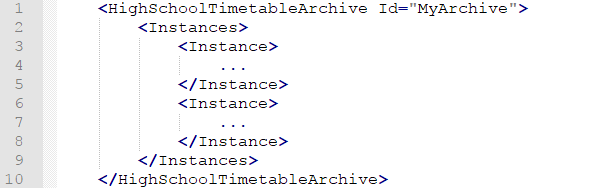
\includegraphics {szablonXHSTTprzyklad}
	\caption{Przykład archiwum w języku XML.}
	\label{fig: Xhsttprzyklad}
\end{figure}

Opcjonalna kategoria \textit{Metadata} zawiera podstawowe informacje na temat archiwum, takie jak: nazwa, autor, data powstania, opis oraz uwagi.

\section{Instancje}

Instancja jest to pojedynczy zestaw danych dla danego problemu układania planu zajęć, najczęściej dla pojedynczej szkoły i konkretnego roku (lub semestru). Składnie instancji zaprezentowano na rysunku 4.3. Wiele kategorii posiada atrybut \textit{Id}, który służy do odnoszenia się do danej kategorii w dalszej części archiwum.

\begin{figure}
	\centering
	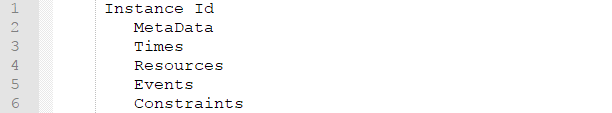
\includegraphics {skladniaSzablon}
	\caption{Szablon pojedynczej instancji.}
	\label{fig: skladniaSzablon}
\end{figure}

\section{Okna czasowe}

Format XHSTT wspiera tylko prosty model czasu, gdzie czas podzielony jest na równe interwały zwane oknami czasowymi. Kategoria \textit{Times} służy do definiowania tych okien. Podkategoria \textit{TimeGroups} definiuje różne grupy czasowe takie jak dni, tygodnie oraz okresy w ciągu dnia. Podkategoria \textit{Time} zawiera definicje okna czasowego, gdzie każde okno oprócz nazwy może mieć przypisany konkretny tydzień, dzień i inne grupy czasowe. Składnia kategorii \textit{Times} wraz z podkategoriami znajduje się na rysunku 4.4. Przykład w języku XML znajduje się na rysunku 4.5. Przedstawia on czwarte okno czasowe w poniedziałek.

\begin{figure}
	\centering
	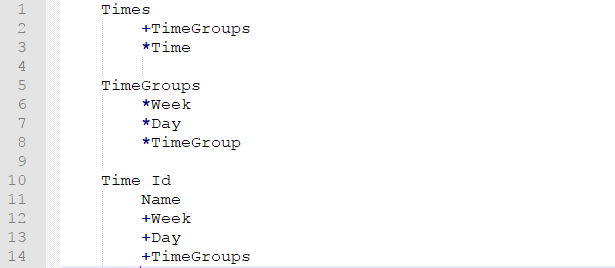
\includegraphics {skladniaTimes}
	\caption{Składnia kategorii: \textit{Times}.}
	\label{fig: skladniaTimes}
\end{figure}

\begin{figure}
	\centering
	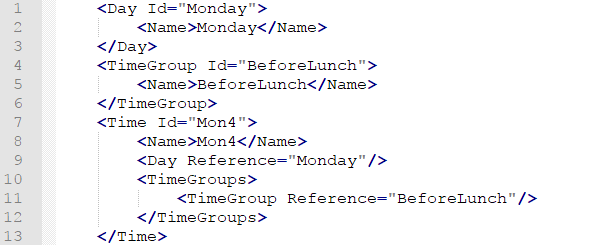
\includegraphics {timesPrzyklad}
	\caption{Przykład deklaracji czwartego okna czasowego w poniedziałek.}
	\label{fig: timesPrzyklad}
\end{figure}

\section{Zasoby}

Zasoby są to wszystkie elementy przypisane do zdarzeń. Do zasobów najczęściej zaliczamy nauczycieli, sale i grupy uczniów, ale format XHSTT dopuszcza dowolne definiowanie zasobów. W skład kategorii \textit{Resources} wchodzą również grupy i typy zasobów. Typ zasobów to np: nauczyciel, sala, grupa. Grupy zasobów gromadzą zasoby jednego typu np: nauczyciele języka polskiego. Składnia kategorii \textit{Resources} zaprezentowana jest na rysunku 4.6, na rysunku 4.7 zaprezentowano przykładową deklarację sali komputerowej.

\begin{figure}
	\centering
	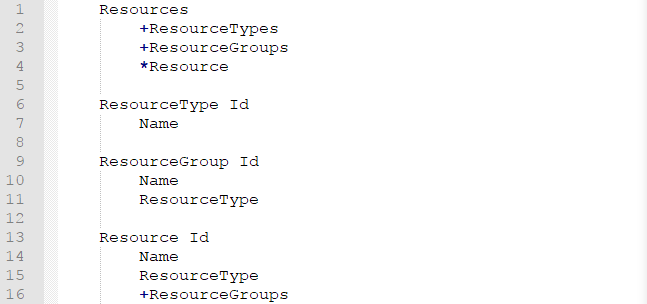
\includegraphics {resourcesSkladnia}
	\caption{Składnia kategorii: \textit{Resources}.}
	\label{fig: resourcesSkladnia}
\end{figure}

\begin{figure}
	\centering
	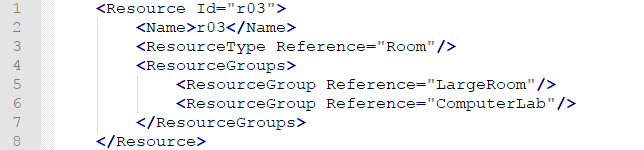
\includegraphics {resourcesPrzyklad}
	\caption{Przykład deklaracji zasobu jako sali komputerowej.}
	\label{fig: resourcesPrzyklad}
\end{figure}

\section{Zdarzenia}

Zdarzenia określone jest jako spotkanie pomiędzy zasobami, czyli w uproszczeniu są to zajęcia odbywające się w konkretnej sali, z konkretnym nauczycielem i grupą studentów. Przed zdarzeniami zdefiniowane mogą być ich grupy, takie jak np. zajęcia z kursu języka obcego. Same zdarzenia zawierają atrybuty określające ich czas trwania oraz termin odbycia się zajęć. Termin odbywania zajęć może być przypisany wcześniej lub może być pozostawiony pusty, w celu przypisania go przez algorytm układający plan zajęć. Dodatkowo zdarzenia posiadają parametr określający kolor zajęć wyświetlany na ułożonym planie. Składnia kategorii \textit{Events} zaprezentowana jest na rysunku 4.8, na rysunku 4.9 zaprezentowano przykładową deklarację zajęć z języka angielskiego.

\begin{figure}
	\centering
	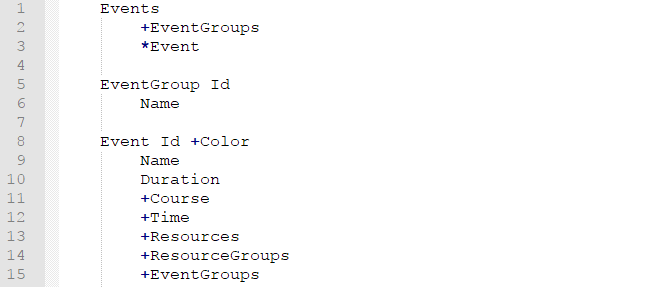
\includegraphics {eventsSkladnia}
	\caption{Składnia kategorii: \textit{Events}.}
	\label{fig: eventsSkladniakladnia}
\end{figure}

\begin{figure}
	\centering
	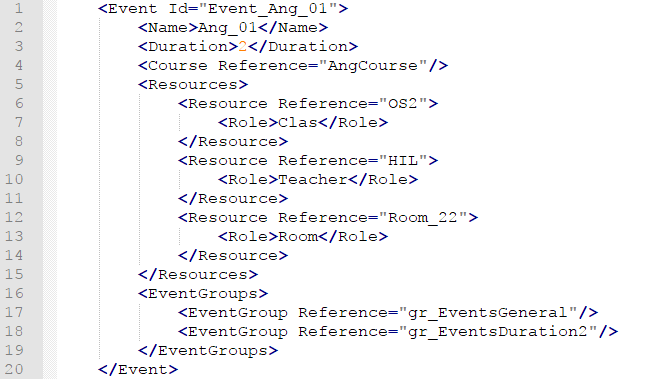
\includegraphics {eventsPrzyklad}
	\caption{Przykład deklaracji zajęć języka angielskiego.}
	\label{fig: eventsPrzyklad}
\end{figure}

\section{Ograniczenia}

Format XHSTT pozwala definiować wiele ograniczeń planu zajęć. Wszystkie one opisane są szczegółowo na stronie internetowej \cite{ograniczenia}. W pracy zostały opisane tylko te, które są uwzględnione w implementacji. Ogólna składnia ograniczenia przedstawiona jest na rysunku 4.10. Każde z ograniczeń ma zdefiniowaną swoją wagę oraz sposób wyliczania funkcji kosztu (liniowa, kwadratowa). Każde ograniczenie jest rozdzielone na ograniczenie twarde lub miękkie poprzez parametr \textit{Required}.

\begin{figure}
	\centering
	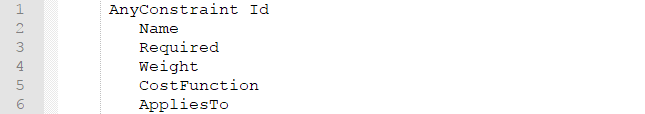
\includegraphics {ograniczeniaSkladnia}
	\caption{Składnia kategorii: \textit{Constraints}.}
	\label{fig: ograniczeniaSkladnia}
\end{figure}

\subsection{Przypisany czas}

Ograniczenie \textit{Assign time constraints} określa, że każde zdarzenie musi mieć przypisany czas oraz definiuje koszt złamania tego ograniczenia. Może być przypisane do wszystkich wydarzeń lub tylko do wybranych grup. Przykład przedstawiono na rysunku 4.11.

\subsection{Unikanie konfliktów}

Ograniczenie \textit{Avoid clashes constraints} określa, czy dane zasoby mogą być podzielone. To znaczy, czy nie są przypisane do dwóch lub więcej zdarzeń odbywających się w tym samym czasie. Jest to ograniczenie stosowane powszechnie, jednak mogą zdarzyć się przypadki, że układający dopuszcza odbywanie się dwóch zajęć w jednej sali jednocześnie (np. zajęcia wychowania fizycznego).

\subsection{Podział zdarzeń}

Ograniczenie \textit{Split events constraints} określa, czy zdarzenia o długości dłuższej niż jeden mogą zostać podzielone i rozłożone na kilka dni. Ograniczenie to pozwala nam definiować minimalne i maksymalne długości bloków jednego zdarzenia.

\subsection{Limit bezczynności}

Ograniczenie \textit{Limit idle times constraints} określa, czy mogą występować i jak długie są dopuszczalne przerwy między zajęciami. Określają, czy pomiędzy dwoma zajęciami jednego dnia, może wystąpić jedno lub więcej nieprzypisanych okien czasowych.

\begin{figure}
	\centering
	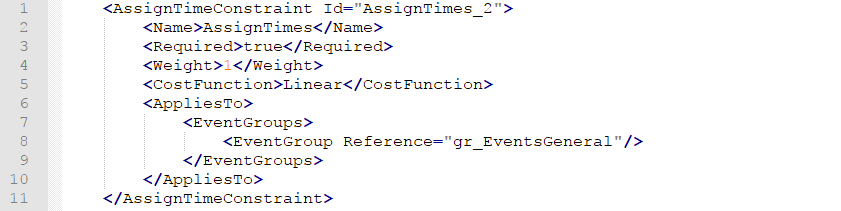
\includegraphics {ograniczeniaPrzyklad}
	\caption{Przykład ograniczenia: \textit{Assign time constraints}.}
	\label{fig: ograniczeniaPrzyklad}
\end{figure}